	\chapter{Sélection de variables via Forets Aléatoire}
	\section{Introduction aux forêts de décision aléatoires}
	Considérons un ensemble d'apprentissage ${L_n = \{(X_1, Y_1),...,X_n, Y_n)\}}$ de \textit{n} observations i.i.d.\footnote{indépendantes identiquement distribuées} d'un vecteur aléatoire (X,Y). Le vecteur ${X_i = (X_i^1,...,X_i^p)}$ contient les variables exogènes, $X_i \in \reels^p $ et $Y_i \in \reels $, une réponse numérique. Pour les problèmes de regression, nous supposons que $ \exists$ S $\forall$ i $ Y_i=S(X_i)+\varepsilon$ où E[$\varepsilon$|X] = 0 et \textbf{S} est appellée fonction de regression. Les FA est une stratégie de construction d'un modèle \textit{ê(x)} estimant la fonction de regression.
	\par
	Les méthodes d’agrégation consistent à agréger un nombre \textit{B} d’estimateurs $ê_1,...,ê_\textit{B}$ : ${ê(x) = ê_B(x) =  \frac{1}{B} \sum_{i=1}^{B} ê_i}$. On considère l’erreur quadratique moyenne d’un estimateur \textit{ê} et sa décomposition biais-variance :
	\begin{center}
	${E[(ê(x)-S(x))^2] = (E[ê(x)] - S(x))^2 + Var(ê(x))}$
	\end{center}
	Si on suppose les régrésseurs $ê_1,...,ê_B$ i.i.d on a :
	\begin{center}
		$E[ê(x)] = E[ê_1(x)]$ et $Var(ê(x)) = \frac{1}{B} Var(ê_1(x)$
	\end{center}
	Le biais de l’estimateur agrégé est donc le même que celui des $ê_k(x)$ mais la variance diminue. Bien
	entendu, en pratique il est quasiment impossible de considérer des estimateurs $ê_k(x)$ indépendants
	dans la mesure où ils dépendent tous du même échantillon \textit{$L_n$} . L’approche des FA consiste à
	tenter d’atténuer la dépendance entre les estimateurs que l’on agrège en les construisant sur des
	échantillons bootstrap\footnote{Ré-échantillonnage}. Nous référerons le lecteur à l'annexe A4, pour une démonstration.


\section{Utilisation de CART dans la construction des Forêts aléatoires}
En comparaison avec le modèle CART qui lui procède à une phase de construction de l'arbre suivie d'une phase d'élagage, deux différences sont à relever. D'abord, à chaque nœud, un nombre paramètre (dénoté \textit{k}\footnote{L'autre paramètre des FA étant \textit{B}, le nombre d'arbres dont la forêt.}) de variables exogènes sont choisies aléatoirement et la meilleure variable pour la subdivision du nœud est choisie parmi celles-ci seulement. Ensuite, aucun élagage n'est introduit: tous les arbres de la forêt sont maximaux.\par
	Le principe de CART est de partitionner récursivement l’espace engendré par les variables explicatives (ici $\reels^p$) de façon dyadique. Plus précisément, à
	chaque étape du partitionnement, on découpe une partie de l’espace en deux sous parties selon une variable $X_j$ comme le montre la figure \ref{fig:CART}.
	\begin{figure}[h]
	    		\centering
	    		\fbox{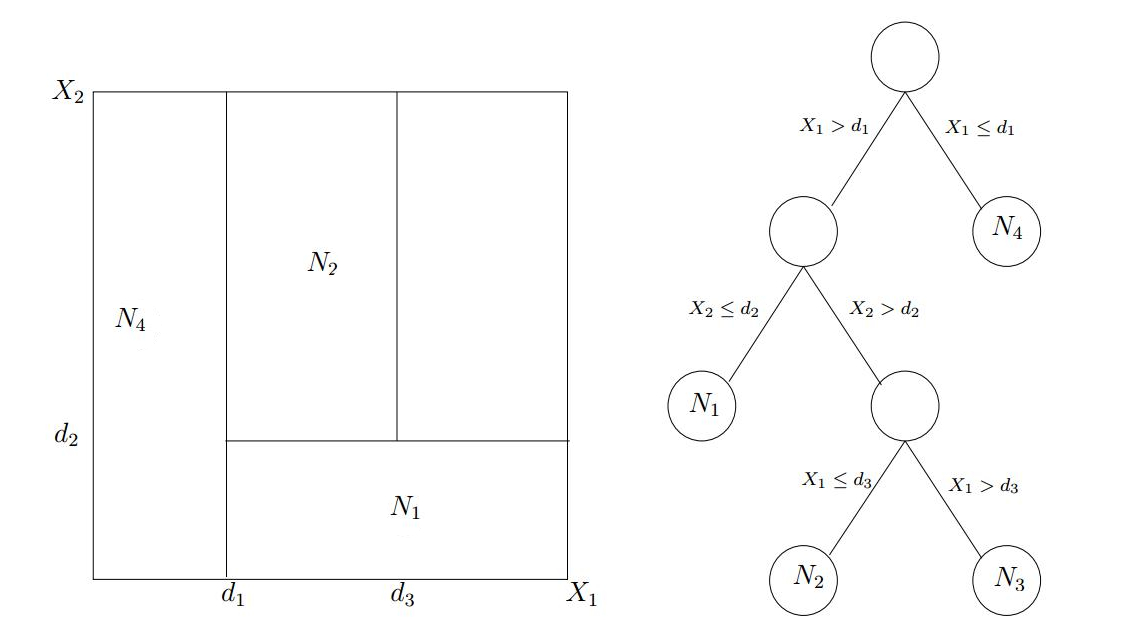
\includegraphics[width=\textwidth]{Cart}}
	    		\caption{Arbre CART}
	    		\label{fig:CART}
	\end{figure}
	\par
	Les coupures sont choisies de manière à minimiser une fonction de coût particulière. A chaque étape, on cherche la variable $X_j$ et le réel \textit{d} qui minimisent la variance des nœuds fils dans les problèmes de régression. Les arbres sont ainsi construits jusqu’à atteindre une règle d’arrêt. Par exemple, on ne découpe pas un nœud qui contient moins de 5 observations comme y procède le package \textbf{\textit{randomForest}} du langage \textbf{R}.\par
	L'agrégation à laquelle procèdent les FA est d’autant plus performante que la corrélation entre les prédicteurs agrégés  (arbres CART) est faible. Afin de diminuer cette corrélation, Breiman\cite{BREI01} propose de rajouter une couche d’aléa dans la construction des
		prédicteurs. Plus précisément, à chaque étape de CART, \textit{k} variables sont sélectionnées aléatoirement parmi les \textit{p} et la meilleure coupure est sélectionnée uniquement sur ces \textit{k} variables. \par
		On retrouve un compromis biais-variance dans le choix de m :
		\begin{itemize}
		\item lorsque \textit{k} diminue, la tendance est à se rapprocher d’un choix aléatoire des variables
		de découpe des arbres. Dans le cas extrême où \textit{k} = 1, les axes de la partition des arbres
		sont choisies au hasard, seuls les points de coupure utiliseront l’échantillon. Ainsi, si \textit{k}
		diminue, la corrélation entre les arbres va avoir tendance à diminuer également, ce qui
		entraînera une baisse de la variance de l’estimateur agrégé. En revanche, choisir les axes
		de découpe des arbres de manière aléatoire va se traduire par une moins bonne
		qualité d’ajustement des arbres sur l’échantillon d’apprentissage, d’où une augmentation
		du biais pour chaque arbre ainsi que pour l’estimateur agrégé.
		\item lorsque \textit{k} augmente, les phénomènes inverses se produisent.
		\end{itemize}
		On déduit de cette remarque que le choix de \textit{k} est lié aux choix des paramètres de l’arbre,
		notamment au choix du nombre d’observations dans ses nœuds terminaux. En effet, si ce
		nombre est petit, chaque arbre aura un biais faible mais une forte variance. Il faudra dans ce cas là s’attacher à diminuer cette variance et on aura donc plutôt tendance à choisir une
		valeur de \textit{k} relativement faible. A l’inverse, si les arbres ont un grand nombre d’observations
		dans leurs nœuds terminaux, ils posséderont moins de variance mais un biais plus élevé. Dans
		ce cas, la procédure d’agrégation se révélera moins efficace. C’est pourquoi, en pratique, le
		nombre maximum d’observations dans les nœuds est par défaut pris relativement petit (5). Concernant le choix de \textit{k}, \textit{\textbf{randomForest}} propose par
		défaut \textit{k = $\frac{p}{3}$} en régression. Ce paramètre peut également
		être sélectionné via des procédures apprentissage-validation ou validation croisée.
		
		
		\section{L'erreur Out-Of-Bag et le score FA d'importance des variables}
\paragraph{L'erreur Out Of Bag:}
	Il s'agit d'une procédure permettant de fournir un estimateur de l'erreur ${E[(\hat{e}(x)-Y)^2]}$ en régression. De tels estimateurs sont souvent construits à l'aide de méthode apprentissage-validation ou validation croisée. L'avantage de la procédure Out Of Bag (OOB) est qu'elle ne nécessite pas de découper
	l'échantillon. Elle utilise le fait que les arbres sont construits sur des estimateurs agrégés et que,
	par conséquent, ils n'utilisent pas toutes les observations de l'échantillon d'apprentissage. Étant donné une observation ${(X_w,Y_w)}$ de $L_n$, on désigne par ${\omega_B}$ l'ensemble des arbres de la forêt qui
	ne contiennent pas cette observation dans leur échantillon bootstrap. Pour estimer, la prévision de
	la forêt sur ${Y_w}$ on agrège uniquement ces arbres là :
	\begin{center}
	$\hat{Y}_w = \frac{1}{|\omega_B|} \sum_{i \in \omega_B} ê(X_w,\theta_i)$
	\end{center}
\paragraph{L'importance des variables:}
	L'inconvénient des méthodes d'agrégation est que le modèle construit est difficilement interprétable, on parle souvent d'aspect boite noire.
	pour ce type de méthodes. Pour le modèle de forêts aléatoires que nous venons de présenter,
	Breiman\cite{BREI01} propose une mesure qui permet de quantifier l'importance des variables $X_j$, j=1,...,p dans le modèle.
	On désigne par $OOB_k$ l'échantillon Out Of Bag associé au \textit{k}$^{ème}$ arbre de la forêt. Cet échantillon est formé par les observations qui ne figurent pas dans le \textit{k}$^{ème}$ échantillon bootstrap. On note $E_{OOB_k}$ l'erreur de prédiction de l'arbre $ê(.,\theta_k)$ mesurée sur cet échantillon :
	\begin{center}
	$E_{OOB_k} = \frac{1}{|OOB_k|} \sum_{i \in OOB_k} (ê(X_i,\theta_k) -Y_i)^2.$
	\end{center}
	On désigne maintenant par $OOB_{k}^{j}$ l'échantillon $OOB_k$ dans lequel on a perturbé aléatoirement
	les valeurs de la variable \textit{j} et par $E_{OOB_{k}^{j}}$ l'erreur de prédiction de l'arbre $ê(.,\theta_k)$ mesurée sur cet échantillon :
	\begin{center}
		$E_{OOB_{k}^{j}} = \frac{1}{|OOB_{k}^{j}|} \sum_{i \in OOB_{k}^{j}} (ê(X_{i}^{j},\theta_k) -Y_i)^2.$
	\end{center}	
	où les $X_{i}^{j}$ désignent les observations perturbées de $OOB_{k}^{j}$. Empiriquement, si la \textit{j}$^{ème}$ variable joue un rôle déterminant dans la construction de l'arbre $ê(.,\theta_k)$, alors une permutation de ces valeurs \textit{j} dégradera fortement l'erreur. La différence d'erreur $E_{OOB_{k}^{j}}$ - $E_{OOB_k}$ sera alors élevée. L'importance de la \textit{j}$^{ème}$ variable sur la forêt est mesurée en moyennant ces différences d'erreurs sur tous les arbres :
	\begin{center}
	${Imp(X_j) = \frac{1}{B} \sum_{k=1}^{B} (E_{OOB_{k}^{j}} - E_{OOB_k}) }$
	\end{center}
	
	
	\section{Étude du biais et de variance d'un estimateur agrégé \cite{ESL}}
	\begin{small}
	Comparons le biais et la variance de l’estimateur agrégé à ceux des estimateurs que l’on agrège.
	Le fait de considérer des échantillons bootstrap introduit un aléa supplémentaire dans l’estimateur. Afin de prendre en compte cette nouvelle source d’aléatoire, on note $\theta_k = \theta_k(L_n)$ l’échantillon bootstrap de \textit{k} variables exogènes à l’étape \textit{i} et ê($\theta_k$) l’estimateur construit. On écrira l'estimateur final ${ê_B(x) =  \frac{1}{B} \sum_{i=1}^{B} ê_i(x,\theta_k)}$
	\par
	Les tirages bootstrap sont effectués de la même manière et indépendamment les uns des autres.
	Ainsi, conditionnellement à $L_n$ , les variables $\theta_1,..., \theta_B$ sont i.i.d. et de même loi que $\theta$ (qui représentera la loi de la variable de tirage de l’échantillon bootstrap. Ainsi, d’après la loi des grands nombres :
	\begin{center}
		${ê(x) = \lim_{B \to \infty} ê_B(x) = \lim_{B \to \infty} \frac{1}{B} \sum_{i=1}^{B} ê_i(x,\theta_k) = E_\theta[ê(x,\theta) | L_n]  }$
	\end{center}
	L’espérance est ici calculée par rapport à la loi de $\theta$. Prendre \textit{B} trop grand ne va pas sur-ajuster l’échantillon, autrement dit prendre la limite en \textit{B} revient à considérer un estimateur “moyen” calculé sur tous les échantillons bootstrap. Le choix de \textit{B} n’est donc pas crucial pour la performance de l’estimateur, il est recommandé de le prendre le plus grand possible. On note :
	\begin{itemize}
	\item ${T_k=ê(x,\theta_k)}$, les estimateurs que l'on agrège, ceux ci étant identiquement distribués.
	\item ${\sigma^2(x) = Var (T_k)}$, la variance des estimateurs que l'on agrège.
	\item ${\rho(x) = corr[T_1,T_2]}$, le coefficient de corrélation entre deux estimateurs que l’on agrège (calculés sur deux échantillons bootstrap).
	\end{itemize}
	La variance ${\sigma^2(x)}$ et la corrélation ${\rho(x)}$ sont calculées par rapport aux lois de \textit{$L_n$} et de $\theta$. On suppose que les estimateurs sont identiquement distribués. Il est alors facile de voir que le biais
	de l’estimateur agrégé est le même que le biais des estimateurs que l’on agrège. Par conséquent,
	agréger ne modifie pas le biais. Pour la variance, on a le résultat suivant:
	\begin{equation*}
	\begin{split}	
	Var(ê_B(x)) = Var [ \frac{1}{B} \sum_{i=1}^{B} T_i] = \frac{1}{B^2} [\sum_{i=1}^{B} Var(T_i) + \sum_{1 \leq i \neq i' \leq B} cov(T_i,T_{i'}) ] \\ = \frac{1}{B}\sigma^2(x) + \frac{1}{B^2}[B^2-B]\rho(x)\sigma^2(x) = \rho(x)\sigma^2(x) + \frac{1-\rho(x)}{B}\sigma^2(x)
	\end{split}
	\end{equation*}

	Ainsi, si $\rho(x)$ < 1, l’estimateur agrégé a une variance plus petite que celle des estimateurs que l’on
	agrège (pour \textit{B} suffisamment grand). On déduit que c’est la corrélation $\rho(x)$ entre les estimateurs que l’on agrège qui quantifie le gain de la procédure d’agrégation : la variance diminuera d’autant plus que les estimateurs que l’on agrège seront décorrélés. Le fait de construire les estimateurs sur des échantillons bootstrap va dans ce sens.
		\end{small}
		
